%@+leo-ver=4-thin
%@+node:hasletpara.20131129101631.1917:@shadow ./fmpp/Tex/Thesis/thes.tex
%@@color
%@@language latex

\documentclass[12pt, a4paper, twoside, openright]{book}

\usepackage{vuwthesis} % sets up some local things, mostly the front page

\usepackage{palatino} % sets palatino as the default font

\usepackage{url} % for typesetting urls



%\renewcommand{\baselinestretch}{1.00}


\begin{document}

\frontmatter
% Book style knows about front matter
% Report style doesn't so you need to set roman numbering etc yourself :-(

%%%%%%%%%%%%%%%%%%%%%%%%%%%%%%%%%%%%%%%%%%%%%%%%%%%%%%%

\title{Maintaining differently refactored views in Java}
\author{Paran Haslett}

\subject{Computer Science}
\abstract{
%@<<abstract>>
%@+node:hasletpara.20131129101631.1918:<<abstract>>
When developers collaborate on a project there are times when the code diverges. This could be due to refactoring or the code being reused in another project. It could even be due to throw away code or code used for debugging. This could at times also involve how the structure of the program is presented or the variable and method names that are being used. This is especially true if there is a piece of functionality that you wish to work on that differs from what everyone else is working on. In these cases you may need to refactor the code to best suit your changes before you apply them. The ability to have a separate view which although functionally equivalent to other views can present the code in a different form in these situations would be valuable. It enables the programmer to refactor or change the code with minimal impact on others. If the relationships between views are maintained it also could better recognise the changes that need to be communicated to other views or branches.
%@nonl
%@-node:hasletpara.20131129101631.1918:<<abstract>>
%@nl
}
% Books don't normally have abstracts, and this is a bit of a hack

% Uncomment the appropriate degree
%\phd
\mscthesisonly
%\mscwithhonours
%\mscbothparts
% \otherdegree{DEGREE OR DIPLOMA NAME}



%%%%%%%%%%%%%%%%%%%%%%%%%%%%%%%%%%%%%%%%%%%%%%%%%%%%%%%




\maketitle


\chapter*{Acknowledgments}\label{C:ack} 

I would like to acknowledge the invaluable help of both my supervisors David Pearce and Lindsay Groves and also my wife Hye Eun Park who has been a great support during this thesis.


\tableofcontents


%%%%%%%%%%%%%%%%%%%%%%%%%%%%%%%%%%%%%%%%%%%%%%%%%%%%%%%

% book style knows about mainmatter
% if you are using report style you will have to rest page numbering etc.
\mainmatter

%%%%%%%%%%%%%%%%%%%%%%%%%%%%%%%%%%%%%%%%%%%%%%%%%%%%%%%

% individual chapters included here


\chapter{Introduction}\label{C:intro}

According to Bertino \cite{Bertino2012} \emph{Version control systems} provide a way of allowing multiple developers to collaborate. When multiple developers work on the same source code there is a risk that they have conflicting changes for the same portion of the source code.  One way of managing these conflicting changes is by ensuring only one person can edit a file at a time. This locking mechanism was recommended by Tichy \cite{Tichy1982} for the RCS version control system. Of course, the problem here is that one person can stop others from being able to edit the file. 

An alternative approach is to allow multiple changes to a file and to automatically resolve most of them in a process called a \emph{merge}.  The merge process compares the changes made in one version with the changes made on the other version. If the merge process determines that changes can coexist, it creates a merged file that contains all the changes. The changes that cannot be automatically merged are known as \emph{merge conflicts}.  The merge conflicts need to be manually checked and edited to form a merged file with the correct changes.

\begin{figure}[!t]
 \begin{center}
 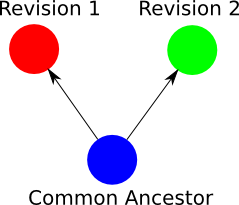
\includegraphics[scale=1]{introRevisions}
 \end{center}
 \caption{A file that has two different revisions}
 \label{fig:introRevisions}
\end{figure}



Internally the merge process needs to determine what changes have happened to both of the revisions being compared. In Figure  ~\ref{fig:introRevisions} there are two revisions that are derived from a common ancestor. It is possible to determine what has been deleted, inserted or changed by comparing each of the revisions against the common ancestor.  This is often done as a linear comparison of the source code for each revision. This works very well provided there has been no change in the order or structure of the file. However, if there has been a change where a block of source code has been moved from one place to another a linear comparison instead determines that two changes have occurred.  This is equivalent to deleting a block of source code from the common ancestor and inserting that source code elsewhere. It is possible that this change is not important to other programmers as the program behaves in the same manner even when source code is in a different order.  An example of this is if a Java programmer changes the order of methods within a program.  The program will behave in the same way as changing the order of methods does not change any functionality, however the source code is now different. The swapping of the order of the method is still counted as being two different changes even though the program behaves in the same manner as it did before the change took place.

Without any further analysis this change is recorded in the merged file even if the reordering was a personal preference for the programmer.  Although there has been no functional change the version control system will treat the relocation of blocks of source code exactly like a change in functionality.  Whenever a programmer attempts to update their code to incorporate any change in functionality, the change to the order of methods is also made to their code.  If a programmer is already familiar with the old structure of code and expects the code to remain relatively consistent the swapping of methods could be disconcerting.

Another issue that non-functional changes raise is an increase in the number of \emph{merge conflicts}. This could occur when two views have had a small amount of refactoring.  Since in both views the behaviour of the program has not changed it is possible that the merge conflict occurs about something trivial. An example of this could be different formatting or ordering methods alphabetically. For an ordinary text merge these changes to the structure of the source code require manual intervention. These issues highlight the need to develop smarter ways to merge.

It is becoming more important to have smarter merges because of the scale of many software projects and the number of developers working on them.
Large online repositories, like GitHub, contain many open source projects.
It is possible for these projects to make source code available to many developers at a time.
This means it is possible for two developers to work on the same project while having little personal contact.
Care needs to be taken when their individual work is combined.
Preferably most of the problems with merging their work should be automatically resolved however,
there still could be instances where either or both developers will have to figure out how the code should interact.
Having better automatic merges reduces the risk that time will be spent manually figuring out how different changes should be combined.

This thesis introduces the concept of maintaining multiple separate views which can be ordered differently but have functionally equivalent source code.
The purpose of these views is to reduce the number of changes introduced during a merge. 
It also explores a way of allowing a version control system to detect when there is a change in the source code but not a functional change in a program.
Examples of this are if items have been reordered, if comments have been inserted or there have been changes to the formatting. 
We developed the Refactor Categories Tool for the purpose of identifying these changes. 
We report on the design and implementation of this tool.
The Refactor Categories Tool is then used in an experiment evaluating a range of real-world benchmarks.


% We have used the Refactor Categories Tool we have created in an experiment 
% that iterates though all the revisions in the version source control for a 
% handful of Java projects.
% The Refactor Categories Tool detects
% 
% need to write about what we found here
 

\section{Overview}
In Chapter 2 we go over the background of version control, the longest common subsequence problem and refactoring as well as look at JDime, an existing tool for merging refactored views.
In Chapter 3 we discuss private views and what they could mean
In Chapter 4 we examine the Refactor Categories Tool, a precursor to developing private view. This will allow us to evaluate if additional merge operations are possible
In Chapter 5 we evaluate the results produced from the Refactor Categories Tool and determine what this could mean for our concept of private views.
In Chapter 6 we will conclude with some future work to make the concept of private view possible. 

% In this thesis we explore the idea of having private views that although 
% functionally equivalent can be refactored differently.
% A version control system allows us to have
% In this thesis we will examine the effects of non functional changes caused 
% by light weight refactoring of code on version control systems.
% To do this we will examine version control systems and how they allow 
% collaboration through merging.
% We will also examine refactoring and how it can change the code but retain 
% the same behaviour.
% We will some tools that could help when merging refactored code when it is 
% checked into an operating system.
% We especially focus on JDime to see if I can help us to build a private view 
% where external code changes are minimised.

\chapter{The front pages}\label{C:ex}

You can declare:
\begin{itemize}
\item an author using  \verb+\author{}+ -- your full name;
\item a title using \verb+\title{}+-- ALL IN CAPITALS IN THE EXAMPLE, but we use \verb#\Large# and \verb#\bf#, so normal case will do;
\item a subject using \verb+\subject{}+-- probably Computer Science, but you can pick anything you like;
\item an abstract using \verb+\abstract{}+-- this should be fewer then 500 words for a PhD. The handbook states ``A length of about 300 words is recommended.'' The \textsf{book} style does not have an \verb+abstract+ environment defined, so this is a bit of a hack.
\end{itemize}

You can also specify what degree you are submitting the thesis for by using:
\begin{itemize}
\item  \verb+\phd+, which produces ``\ldots in fulfilment of \ldots Doctor of Philosophy''
\item  \verb+\mscthesisonly+, which produces ``\ldots in fulfilment of \ldots Master of Science''
\item  \verb+\mscwithhonours+, which produces ``\ldots in partial fulfilment of \ldots Master of Science with Honours''
\item  \verb+\mscbothparts+, which produces ``\ldots in partial fulfilment of \ldots Master of Science''
\item  \verb+\otherdegree{DEGREE OR DIPLOMA NAME}+, which produces ``\ldots in fulfilment of \ldots DEGREE OR DIPLOMA NAME''
\end{itemize}

\chapter{Library requirements}\label{C:lib}

This Chapter describes some things done to be in accordance with the `Library Requirements for the Deposit of Theses' booklet, which can be obtained from the VUW library.

\section{Font size}
\textit{12 point font is recommended.} 

Set this yourself with the \verb+12pt+ option to the document class.

\section{Single or double sided}
\textit{Typing on one side preferred, text on both sides acceptable for longer works.} 

Use the \verb+oneside+ or \verb+twoside+ option to the document class. The \textsf{book} class default is \verb+twoside+.


\section{Line spacing}
\textit{Lines should be double spaced, or at least 1.5 spaces apart.} 

1.5 spacing for 12 point is set using:
\begin{itemize}
\item \verb+\renewcommand{\baselinestretch}{1.24}+  
\end{itemize}

To set anything else use, e.g  \verb+\renewcommand{\baselinestretch}{1.0}+ in the preamble. See p 53 of \cite{GMS94} for more information.


\section{Margins}
\textit{Uniform margins of at least 4cm on binding side, other three sides to have at least 1.5 cm}

\LaTeX\ styles often leave a lot of white space, and \textsf{book} is no exception. We only have to worry about the binding side.

For \verb+twoside+ we use these settings:
\setlength{\textheight}{19.8cm}
\setlength{\oddsidemargin}{1.46cm}
\setlength{\evensidemargin}{0.83cm}

For \verb+oneside+, if we use:
\begin{verbatim}
\setlength{\textheight}{19.8cm}
\setlength{\oddsidemargin}{1.46cm}
\end{verbatim}

Then \textsf{book} gives a margin of 4cm on the binding side, and about 3.2cm elsewhere.

If you want to change these then use the \textsf{layout} package.

\section{Paper size}
\textit{High quality A4 paper, all pages of equal size}

Set this yourself with the \verb+a4paper+ option to the document class.
\chapter{Binding}\label{C:bin}

The Library states:
\begin{itemize}
\item Thesis must be fully bound and cased in cloth or buckram in optional colour. (I think they mean you can pick the colour!)
\item Author's surname and initials and (short) title lettered on spine. (The thesis's title, not the author's, presumably.)
\item Author's full name and full title lettered on front cover. (Again, the thesis's title, not the author's, presumably.)
\item Two copies of a PhD thesis and one copy of a Master's thesis must be deposited. A signed availability slip must accompany the thesis.
\item  The principal supervisor is responsible for the deposit.
\end{itemize}
\chapter{Lorem ipsum}
The following comes from \url{http://www.lipsum.com/} (March 2003).

\section{The standard Lorem Ipsum passage, used since the 1500s}
``Lorem ipsum dolor sit amet, consectetur adipisicing elit, sed do eiusmod tempor incididunt ut labore et dolore magna aliqua. Ut enim ad minim veniam, quis nostrud exercitation ullamco laboris nisi ut aliquip ex ea commodo consequat. Duis aute irure dolor in reprehenderit in voluptate velit esse cillum dolore eu fugiat nulla pariatur. Excepteur sint occaecat cupidatat non proident, sunt in culpa qui officia deserunt mollit anim id est laborum.'' 

\section{Section 1.10.32 of ``de Finibus Bonorum et Malorum'', written by Cicero in 45 BC} 
``Sed ut perspiciatis unde omnis iste natus error sit voluptatem accusantium doloremque laudantium, totam rem aperiam, eaque ipsa quae ab illo inventore veritatis et quasi architecto beatae vitae dicta sunt explicabo. Nemo enim ipsam voluptatem quia voluptas sit aspernatur aut odit aut fugit, sed quia consequuntur magni dolores eos qui ratione voluptatem sequi nesciunt. Neque porro quisquam est, qui dolorem ipsum quia dolor sit amet, consectetur, adipisci velit, sed quia non numquam eius modi tempora incidunt ut labore et dolore magnam aliquam quaerat voluptatem. Ut enim ad minima veniam, quis nostrum exercitationem ullam corporis suscipit laboriosam, nisi ut aliquid ex ea commodi consequatur? Quis autem vel eum iure reprehenderit qui in ea voluptate velit esse quam nihil molestiae consequatur, vel illum qui dolorem eum fugiat quo voluptas nulla pariatur?'' 

\section{1914 translation by H. Rackham} 
``But I must explain to you how all this mistaken idea of denouncing pleasure and praising pain was born and I will give you a complete account of the system, and expound the actual teachings of the great explorer of the truth, the master-builder of human happiness. No one rejects, dislikes, or avoids pleasure itself, because it is pleasure, but because those who do not know how to pursue pleasure rationally encounter consequences that are extremely painful. Nor again is there anyone who loves or pursues or desires to obtain pain of itself, because it is pain, but because occasionally circumstances occur in which toil and pain can procure him some great pleasure. To take a trivial example, which of us ever undertakes laborious physical exercise, except to obtain some advantage from it? But who has any right to find fault with a man who chooses to enjoy a pleasure that has no annoying consequences, or one who avoids a pain that produces no resultant pleasure?'' 

\section{Section 1.10.33 of ``de Finibus Bonorum et Malorum'', written by Cicero in 45 BC}
``At vero eos et accusamus et iusto odio dignissimos ducimus qui blanditiis praesentium voluptatum deleniti atque corrupti quos dolores et quas molestias excepturi sint occaecati cupiditate non provident, similique sunt in culpa qui officia deserunt mollitia animi, id est laborum et dolorum fuga. Et harum quidem rerum facilis est et expedita distinctio. Nam libero tempore, cum soluta nobis est eligendi optio cumque nihil impedit quo minus id quod maxime placeat facere possimus, omnis voluptas assumenda est, omnis dolor repellendus. Temporibus autem quibusdam et aut officiis debitis aut rerum necessitatibus saepe eveniet ut et voluptates repudiandae sint et molestiae non recusandae. Itaque earum rerum hic tenetur a sapiente delectus, ut aut reiciendis voluptatibus maiores alias consequatur aut perferendis doloribus asperiores repellat.'' 

\section{1914 translation by H. Rackham} 
``On the other hand, we denounce with righteous indignation and dislike men who are so beguiled and demoralized by the charms of pleasure of the moment, so blinded by desire, that they cannot foresee the pain and trouble that are bound to ensue; and equal blame belongs to those who fail in their duty through weakness of will, which is the same as saying through shrinking from toil and pain. These cases are perfectly simple and easy to distinguish. In a free hour, when our power of choice is untrammelled and when nothing prevents our being able to do what we like best, every pleasure is to be welcomed and every pain avoided. But in certain circumstances and owing to the claims of duty or the obligations of business it will frequently occur that pleasures have to be repudiated and annoyances accepted. The wise man therefore always holds in these matters to this principle of selection: he rejects pleasures to secure other greater pleasures, or else he endures pains to avoid worse pains.'' 

\chapter{Conclusions and future work}\label{C:con}

In this thesis we presented the concept of maintaining private views in Java.
A private view presented here is an environment that allows a developer to import changes they want while avoiding hidden unwanted changes. 
This concept would also allow programmers to implement lightweight refactoring to their tastes, while minimising the impact on others.  
In evaluating what these private view will look like we used version control systems as a starting point.
There are some features of version control systems that already temporarily limit unwanted changes (e.g. branches).
However, during a merge any unwanted refactoring is imported. 
To this end we created the Refactor Categories Tool as a precursor to creating private views. 
This tool analyses the difference between two revisions such as encountered during a commit and identifies some examples of lightweight refactoring.
The way that the Refactor Categories Tool analyses these differences is by first parsing the source for both commits into a Java Abstract Syntax Tree (AST).
Once the AST is populated we then identify which parts of the AST match the differences we want to examine.
We then use the AST to identify additional features that have been changed. 
The features we have focused on are ones that do not change any functionality such as methods being moved or comments being changed. 
The results show that some of these lightweight refactorings are encountered in practice.
As the Refactor Categories Tool is a prototype it did not, unfortunately, select as many as we hoped.
We believe that it is possible to detect many more non-functional changes using more advanced identification algorithms.

\section{Future work}

In order to further the research into private views it would be useful to evaluate how the Refactor Categories Tool could be enhanced to detect more non functional changes. 
In addition to this some other tools could be adapted to create and evaluate the usefulness of private views.  
\subsection{Changes to the Refactor Categories Tool}

There are a number of ways that the Refactor Categories Tool could be changed to discover more moves, and renames:

\begin{itemize}

  \item At the moment the Refactor Categories Tool only examines moves that occur within a class, however, there could be non-functional changes that occur inside a method. 
An example would be if a local variable declaration was moved.
Sometimes this move would have no effect on the code and others it could cause the code to no longer compile.
  
  \item At the moment the refactor categories tool only compares matches within a limited scope (i.e. a class).  
  By allowing the Refactor Categories Tool to check other parts of the code, such as inner classes or even other files may also produce some interesting results.
Although we cannot guarantee that the moves discovered are valid ones this could give us more information about the source code we are examining.

  \item At the moment the Refactor Categories Tool only examines files that have been identified by JGit as being modified or renamed.
In some instances JGit could have incorrectly determined that a file as been deleted and reinserted rather than being renamed or moved.
This could happen easily since during a move or rename the a Java file changes the package reference and class name within a file.
This is especially true if the class has both been renamed and modified.

  \item Revising the scoring system for matching up inserts and deletes may produce some better results.
At the moment modifications are counted as two changes using the scoring system to match inserts and deletes.
Experimenting by reducing this value could improve the number of matches.

\end{itemize}




   

In addition to moves and renames, other lightweight refactoring may be of interest.
One of these are changes to access modifiers.
An example would be if a methods access changes from being private to being public.
Each of the method calls would then need to be rechecked to ensure that the change does not affect functionality.
Due to the possibilities of overloaded methods in Java this would be complicated.

An additional lightweight refactoring that could be considered is code that has been duplicated.
This could be done in a similar manner as how the Refactor Categories Tool check for code that has moved.
If we also check for code that has been modified slightly we may be able to determine that a copy and paste has been used to generate new code.
However, at the moment the Refactor Categories Tool only considers code that has been changed.
If we want to analyse where code has been copied we would need to check the entire source for copies as opposed to just the items that have changed.

Comments could be associated with the AST Node they relate to.  
With this change would be possible to tell if changing a comment should be reflected in other views when there is a source code change. 
This change is difficult as it is hard to tell which block of code the comment refers to.  
One way this could be done would be to associate single-line comments at the end of the line with the AST Node that appears directly before them and other comments with the AST node that appears directly after them.  
This however is only a rough approximation so it may be helpful to also be able to specify exceptions to these rules by using annotations that tie the comment to a block of code. Annotations could also be used to specify how important the comment is.
If the comment is marked as unimportant it would indicate that it still should not be considered a change even if it differs between revisions.

The Refactor Categories Tool could be re-purposed to allow it to be used as a merge tool rather than a comparison tool that we are currently using it for.  
This would bring us a step closer to being able to realise the vision of having better separated private views.  

Performance of Refactor Categories Tool could be further enhanced by only parsing nodes that contain the text change.
This however would require major changes to the parser or rewriting it. There would also be the complexity of figuring out how to only partially parse a source code.
The benefits of rewriting the parser would save memory in addition to speeding up the parsing of Java code into AST nodes.


\subsection{Other lines of enquiry}

There are other tools that could be modified to determine when a refactoring has taken place.

JDime has already been investigates as part of this thesis.
Although JDime cannot recognise changes to comments or white-space it could be re-purposed.
If it could be converted into a comparison tool rather than a merge tool then code that has been refactored differently could be compared without the result being normalised.

According to Pace \cite{Pace} \emph{DiffJ} is able to find the functional differences between two revisions of Java source code.
When computing the difference DiffJ ignores a range of lightweight refactorings such as moved methods, moved imports and the code being reformatted. 
As it ignores comments and white-space however, it will not be able to determine if there have been comment based changes that may be important. 



% 
% future work: by keeping track of equivalences there is no need to retest 
% using the AST
% 



%%%%%%%%%%%%%%%%%%%%%%%%%%%%%%%%%%%%%%%%%%%%%%%%%%%%%%%

% and of course book style knows about backmatter
% \backmatter caused problems with appendices :-(
% and of course report style doesn't
%%%%%%%%%%%%%%%%%%%%%%%%%%%%%%%%%%%%%%%%%%%%%%%%%%%%%%%


%\bibliographystyle{ieeetr}
\bibliographystyle{acm}
\bibliography{Thesis}


\end{document}
%@-node:hasletpara.20131129101631.1917:@shadow ./fmpp/Tex/Thesis/thes.tex
%@-leo
